\documentclass{standalone}
\usepackage{tikz}

\begin{document}
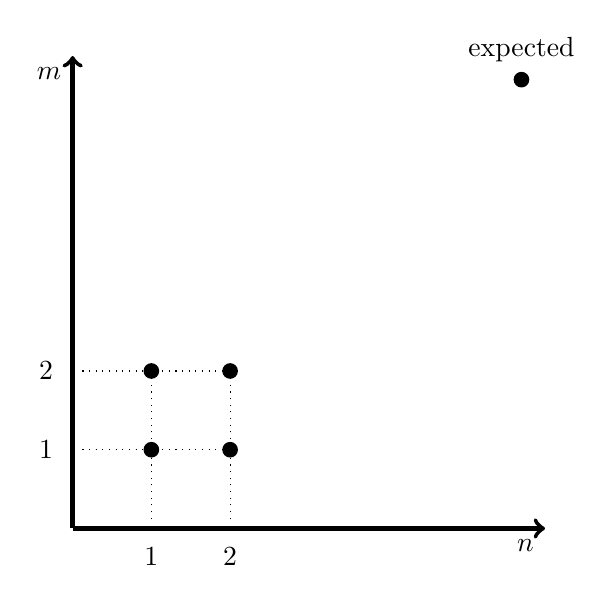
\begin{tikzpicture}
    \draw[->,ultra thick] (0, 0)--(6,0) node[below left]{$n$};
    \draw[->,ultra thick] (0, 0)--(0,6) node[below left]{$m$};
    
    \node[fill, circle, label=above:expected, inner sep=2pt] at (5.7, 5.7) {};
    \node[fill, circle, inner sep=2pt] (stochastic1) at (1, 1) {};
    \node[fill, circle, inner sep=2pt] (stochastic2) at (2, 2) {};
    \node[fill, circle, inner sep=2pt] (stochastic3) at (1, 2) {};
    \node[fill, circle, inner sep=2pt] (stochastic4) at (2, 1) {};

    \node[label=left:1] (y1) at (0, 1) {};
    \node[label=below:1] (x1) at (1, 0) {};

    \draw[dotted] (y1)--(1, 1) {};
    \draw[dotted] (x1)--(1, 1) {};

    \node[label=left:2] (y2) at (0, 2) {};
    \node[label=below:2] (x2) at (2, 0) {};

    \draw[dotted] (y2)--(2, 2) {};
    \draw[dotted] (x2)--(2, 2) {};

    \draw[dotted] (y1)--(2, 1) {};
    \draw[dotted] (x1)--(1, 2) {};

\end{tikzpicture}
\end{document}